\documentclass[11pt]{article}

\usepackage[T1]{fontenc}
\usepackage[utf8]{inputenc}
\usepackage{lmodern}
\usepackage[margin=1in]{geometry}
\usepackage{microtype}
\usepackage{amsmath}
\usepackage{booktabs}
\usepackage{tabularx}
\usepackage{xcolor}
\usepackage{listings}
\usepackage{tikz}
\usetikzlibrary{positioning,arrows.meta,fit,backgrounds}
\usepackage[numbers,sort&compress]{natbib}
\usepackage[hidelinks]{hyperref}
\usepackage{cleveref}
\hypersetup{pdfauthor={dgxcoder}, pdftitle={Mightling: A Vendor-Free Coding Agent on a Single Unified-Memory Workstation}}

\lstset{
  basicstyle=\ttfamily\small,
  columns=fullflexible,
  keepspaces=true,
  breaklines=true,
  frame=single,
  framerule=0.3pt,
  xleftmargin=0.5em,
  xrightmargin=0.5em,
}

\newcommand{\code}[1]{\texttt{#1}}

\title{Mightling: A Vendor-Free Coding Agent on a Single Unified-Memory Workstation, Built on
the Codex CLI}

\author{dgxcoder\\ \texttt{dgxcoder@dreamference.ai}}

\date{October 2026}

\begin{document}
\maketitle

\begin{abstract}
Terminal coding agents such as the Codex CLI are open source, but they are built around a
hosted model, a vendor account and a cloud of companion services. We describe \emph{Mightling}, a
coding agent whose model runs on one NVIDIA GB10 workstation (128\,GB of CPU--GPU unified memory):
a 27B-parameter model (Qwen3.8-27B, NVFP4) served locally through SGLang with a block-diffusion
drafter. Source code, prompts and
inference never leave the machine, and no vendor account is involved. Mightling is a fork of
the Codex CLI (release \code{rust-v0.158.0}, 4{,}894 Rust source files, 1.93 million lines). Its
central engineering choice is to keep the fork almost identical to upstream. The upstream tree is
never edited. Each build exports it, applies a series of 23 patches totalling 42.7\,KB (43 files,
$+169/-53$ lines), and links in a separate crate that does the actual work of localisation: model
discovery, configuration, prompt rebranding, help-text rewriting, a signed release-based updater
and refusal of cloud-bound commands. We report how the series shrank from an initial 406\,KB to
about 9\,KB, which techniques did it, and how seven later features each cost only a hook. We also
report an inventory of the cloud dependencies we had to switch off, a trace-based audit that keeps
them off, an enforced network switch, integration findings that are not visible from the
documentation, and the host-safety layer that unified memory forced on us after model loads froze
the machine. On a 24-task sample of SWE-bench Verified, run inside each task's container on this
machine, the agent resolves a median of 16 tasks over six rounds; calibrated against the 175
published leaderboard submissions on the same tasks, that corresponds to about 71\% on all of
Verified (95\% band 60--81\%), and a two-session ``study, then fix'' mode resolved 20 in its one
round (about 82\%). We then report what was built on the fork, each from the same launcher crate
or beside it: a terse-answer mode that halves answers to questions and leaves coding work
unchanged, a two-layer code index (a tree-sitter knowledge graph plus compiler-exact SCIP data), an
overnight task queue that works in git worktrees, and a client/node split that pairs workstations
over SSH. We are explicit about what is estimated rather than measured.
\end{abstract}

\section{Introduction}

Agentic coding tools now read repositories, run shell commands and edit files autonomously
\cite{yao2023react,yang2024sweagent,wang2024openhands}. The most capable of them are distributed as
open-source clients of proprietary services. The client is inspectable, but a session sends source
code, prompts and tool output to a hosted model. Many organisations cannot accept that. Examples
are regulated industries, security research, and anyone whose code is itself the asset.

Two developments make a local alternative plausible. First, open-weight models in the 100B+
parameter class, quantised to four bits \cite{cheng2023autoround} and accelerated with speculative
decoding \cite{leviathan2023speculative,chen2026dflash}, now generate at interactive speed on a
single desk-side machine. Second, the leading agent clients are open source, so a local deployment
can reuse years of agent engineering rather than rebuild it. Examples of that engineering are the
tool-calling loop, sandboxing, approval flows and the terminal user interface.

Reusing a fast-moving upstream has a cost. A fork that edits the code freely soon stops being able
to take upstream releases. A fork that edits nothing cannot remove the parts that assume a cloud.
This paper reports how we navigated that tension in Mightling, a local AI stack for the NVIDIA GB10
made by Dreamference; its subject is Mightling's terminal coding agent.

\paragraph{What ``local'' means here.} The model, the agent and all session state run on one
workstation. Source code, prompts, tool output and model traffic never leave it, no vendor
account exists, and a traced session shows no connection to any vendor
(\cref{sec:egress}). Mightling is not air-gapped, however. Network access happens only through tools the
agent or user invokes explicitly:
\begin{itemize}
  \item web search goes through a SearXNG \cite{searxng} instance on the machine, which queries
    upstream search engines on the agent's behalf;
  \item reading mail uses Gmail over IMAP, and Drive and Calendar their own read-only APIs;
  \item \code{ling update} contacts GitHub;
  \item building \code{ling} downloads dependencies.
\end{itemize}
Gmail access can be switched off (\code{ling\_gmail = false}), and so can every network access of
the agent: \code{/airgapped on} gives each command the agent runs an empty network namespace
(\cref{sec:egress}). Updates and builds happen only when the user starts them. No model traffic
leaves the machine, with one exception: at the default level, search queries the agent composes go
to upstream engines through SearXNG, and they can contain fragments of code or context.

\paragraph{Contributions.}
\begin{itemize}
  \item A \textbf{patch-minimal fork method} for a large Rust agent (\cref{sec:fork}). The method has
    four parts: an unmodified pinned submodule, a build-time export, a small series of one- and
    two-line hooks, and an external crate linked into the binary. We quantify the result: 42.7\,KB
    of patches against a 1.93M-line upstream, of which the localisation itself took about 9\,KB.
    We also report the techniques that reduced the series from 406\,KB.
  \item An \textbf{inventory of the cloud surface} of a modern coding-agent client, and how each part
    was refused, hidden, replaced or repurposed (\cref{sec:cloud}), with a trace-based audit that
    re-checks it after every build and a network switch enforced in the command sandbox.
  \item \textbf{Integration findings} for running a vendor agent against a local model
    (\cref{sec:local}). They cover discovering the served model, the undocumented catalogue schema,
    a configuration-scoping failure, and why Model Context Protocol tools were invisible to the
    local model until they were flattened into plain functions.
  \item A \textbf{host-safety layer for unified memory} (\cref{sec:safety}). It combines pre-load
    admission checks with a pressure-stall watchdog, and was motivated by real incidents in which
    model loads froze the workstation.
  \item A \textbf{measured cost model for a local agent's output} and the terse-answer mode built on
    it (\cref{sec:local}): on this machine one token of prose costs the time of about 67 prompt
    tokens, and three quarters of the agent's output is tool-call arguments that no speaking style
    touches.
  \item A \textbf{task-level evaluation on SWE-bench Verified} run on an arm64 desk machine
    (\cref{sec:swebench}), with an estimate of the matching overall score calibrated on every
    published leaderboard submission's per-task results.
  \item An \textbf{evaluation} of what exists (\cref{sec:eval}), an implemented code index that
    combines a tree-sitter graph with SCIP and reports which of the two answered
    (\cref{sec:index}), an overnight task queue (\cref{sec:night}), pairing of several workstations
    (\cref{sec:node}), and lessons for fork-based agent products (\cref{sec:lessons}).
\end{itemize}

\section{Background}

\paragraph{The Codex CLI.} The Codex CLI \cite{openai2026codex} is an open-source Rust workspace of about
160 crates. It includes a terminal UI, a non-interactive \code{exec} mode, session
resume and fork, a platform sandbox (Bubblewrap on Linux) and an approval model for tool calls. It
also has \emph{Code Mode}, in which the model is given a single \code{exec} tool and writes short
JavaScript programs. A separate V8-based host process (\code{codex-code-mode-host}) runs these
programs, and within them every other tool, including Model Context Protocol (MCP)
\cite{mcp2025spec} tools, is callable as a function. Codex can talk to ``open-source'' providers
(\code{-{}-oss}) through a standard chat-completions endpoint. Many product surfaces, however, assume an
account with the vendor's hosted service: login, cloud tasks, connectors, usage limits and feedback upload. The
self-updater needs no account, but it installs from the vendor's distribution channels.

\paragraph{The machine.} The NVIDIA GB10 pairs an Arm CPU with a Blackwell GPU (compute capability
12.1) over 128\,GB of shared LPDDR5X. No memory is reserved for the GPU. Model weights, KV cache,
the desktop and every other process draw from the same pool. This one fact shapes much of
\cref{sec:safety}.

\paragraph{The model.} Mightling's default model is Qwen3.8-27B in an NVFP4 checkpoint, served by
SGLang and accelerated by a calibrated NVFP4 DFlash2 block-diffusion drafter
\cite{chen2026dflash,dflash2drafter} that proposes sixteen tokens per step. SGLang serves it
because the drafter runs nowhere else yet. The model runs with a 262k-token context; on the GB10 it
decodes 25.5, 50.3 and 87.0 tokens/s on prose, code and JSON, single-stream, and leaves about
38\,GB of memory free while serving. On real agent sessions, where prompts are long and output is
mostly tool calls, it averages about 30 tokens/s, with about 4.9 of the sixteen drafted tokens
accepted per step. It is the only model served. The default until 2026-09-29 was
Qwen3.5-122B-A10B, a mixture-of-experts model with about 10B parameters active per token, in
Intel's AutoRound int4 checkpoint \cite{qwen35int4,cheng2023autoround} with FP8 dense layers,
served by vLLM \cite{kwon2023vllm} with a twelve-token DFlash drafter \cite{dflashdrafter}. It ran with a 32k-token
context, a limit forced by memory headroom (\cref{sec:safety}), and decoded 23.8, 49.9 and 53.1
tokens/s on the same three kinds of output; it was kept as a fallback until 2026-10-07 and then
removed with its images. The vLLM launcher remains, so the method does not depend on one engine.

\section{System overview}
\label{sec:overview}

\begin{figure}[t]
\centering
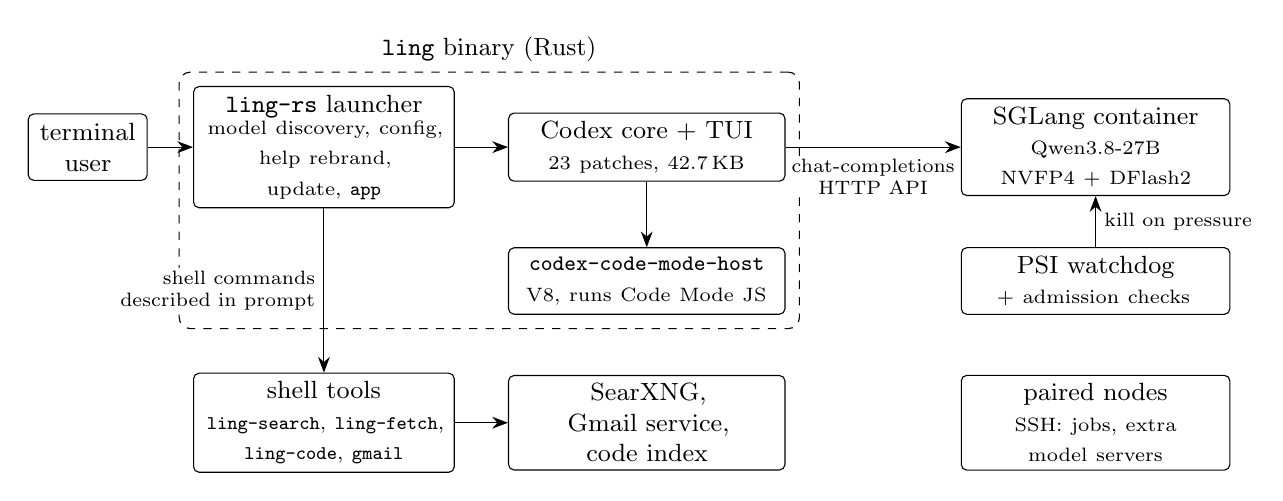
\begin{tikzpicture}[
  box/.style={draw, rounded corners=2pt, align=center, font=\small, inner sep=3pt,
              minimum height=2.4em, text width=#1},
  box/.default=2.6cm,
  grp/.style={draw, dashed, rounded corners=4pt, inner sep=5pt},
  lbl/.style={font=\scriptsize, fill=white, inner sep=1pt},
  >={Stealth[length=2mm]}]
  % row 1: the request path
  \node[box=1.3cm]  (user)     at (-0.2,0)  {terminal\\user};
  \node[box=3.1cm]  (launcher) at (2.8,0)   {\code{ling-rs} launcher\\\scriptsize model discovery, config,\\help rebrand, update, \code{app}};
  \node[box=3.3cm]  (codex)    at (6.9,0)   {Codex core + TUI\\\scriptsize 23 patches, 42.7\,KB};
  \node[box=3.2cm]  (vllm)     at (12.6,0)  {SGLang container\\\scriptsize Qwen3.8-27B NVFP4 + DFlash2};
  % row 2
  \node[box=3.3cm]  (host)     at (6.9,-1.7)  {{\footnotesize\code{codex-code-mode-host}}\\\scriptsize V8, runs Code Mode JS};
  \node[box=3.2cm]  (watch)    at (12.6,-1.7) {PSI watchdog\\\scriptsize + admission checks};
  % row 3
  \node[box=3.1cm]  (tools)    at (2.8,-3.5)  {shell tools\\\scriptsize\code{ling-search}, \code{ling-fetch}, \code{ling-code}, \code{gmail}};
  \node[box=3.3cm]  (svc)      at (6.9,-3.5)  {SearXNG, Gmail service,\\code index};
  \node[box=3.2cm]  (diff)     at (12.6,-3.5) {paired nodes\\\scriptsize SSH: jobs, extra model servers};
  % the binary
  \begin{scope}[on background layer]
    \node[grp, fit=(launcher)(codex)(host), label={[font=\small]above:\code{ling} binary (Rust)}] {};
  \end{scope}
  \draw[->] (user) -- (launcher);
  \draw[->] (launcher) -- (codex);
  \draw[->] (codex) -- (host);
  \draw[->] (codex) -- node[lbl, below=3pt, align=center] {chat-completions\\HTTP API} (vllm);
  \draw[->] (watch) -- node[lbl, right=2pt] {kill on pressure} (vllm);
  \draw[->] (launcher) -- node[lbl, left=2pt, align=right] {shell commands\\described in prompt} (tools);
  \draw[->] (tools) -- (svc);
\end{tikzpicture}
\caption{Mightling at run time. The only Codex code paths that differ from upstream are the hooks
applied by the patch series; everything Mightling-specific lives in the linked \code{ling-rs}
crate or in separate local services.}
\label{fig:overview}
\end{figure}

\Cref{fig:overview} shows the running system. The user types \code{ling}, a single Rust binary.
Before Codex parses its command line, the linked launcher crate runs several steps. It finds the
local model server and waits for it if it is still loading. It asks the server which model it serves
and how long that model's context is. It writes the model catalogue and configuration Codex needs.
Finally it prepends the options that point Codex at the local provider. From then on the process is
Codex, and every upstream flag and subcommand behaves as documented, apart from the cloud surfaces
listed in \cref{sec:cloud}.

Web search and page fetching are two small Rust programs, \code{ling-search} and
\code{ling-fetch}, installed beside \code{ling}; code navigation is a third,
\code{ling-code} (\cref{sec:index}); Gmail reading is provided by
\code{ling-admin}, the Python management CLI. The agent invokes them as shell commands
(\cref{sec:local}). The same \code{ling-admin} manages the model-server container, a browser chat
UI built on Onyx \cite{onyx}, the nightly run of queued tasks (\cref{sec:night}), the pairing of
other workstations (\cref{sec:node}), SWE-bench runs (\cref{sec:swebench}), and the build of
\code{ling} itself. A desktop app (Electron, with \code{ling} bundled) and prebuilt clients for
macOS and Windows reach the same model server over the local network.

\section{A patch-minimal fork}
\label{sec:fork}

\subsection{Build pipeline}

Codex is vendored as a git submodule of our own GitHub fork, pinned to the stable release tag
\code{rust-v0.158.0}. The submodule is \emph{never modified}: the builder's tests assert that
\code{git status} inside it is empty after a build. A build proceeds in six steps.
\begin{enumerate}
  \item Export the pinned commit's \code{codex-rs/} directory with \code{git archive} into a scratch
    tree.
  \item Copy the launcher crate, which is ordinary source in our repository, into that tree as
    \code{codex-rs/ling}.
  \item Apply the patch series with \code{git apply -{}-check} and then \code{git apply}, so a patch
    that no longer fits fails before anything is half-applied.
  \item Build \code{ling} and \code{codex-code-mode-host} with Cargo, into a persistent target
    directory. A persistent target means an edit recompiles only the crates it touches.
  \item Install both binaries side by side, because Codex locates the Code Mode host next to its own
    executable. Symlink \code{\textasciitilde/.local/bin/ling} to the installed binary.
  \item Record a \emph{build key}: a hash of the submodule commit, every patch's bytes, the launcher
    sources and the compiler-profile overrides. An unchanged key skips the build.
\end{enumerate}

The three shell tools are not part of that build. \code{ling-search} and \code{ling-fetch}
share one crate and \code{ling-code} has another, each with its own lockfile, built
\code{-{}-locked} and keyed separately, so changing them never relinks Codex.

Moving to a new upstream release means bumping the submodule and resolving whichever hunks stop
applying. Because the hunks are few and small, conflicts are local and obvious.

\subsection{From 406\,KB to 9\,KB, then features at a hook each}

The first working series had four patches totalling 406{,}116 bytes. \Cref{tab:patches} shows the
current one. Four techniques brought it to about 9\,KB.

\paragraph{Rename at run time, not in the tree.} 395{,}156 bytes of the original series came from a
single patch renaming the agent in Codex's bundled model catalogue (\code{models.json}). That file
stores each system-prompt template, about 20\,KB, as one JSON line, so a one-word change produces a
whole-line diff. The launcher now reads the bundled catalogue through the upstream crate's public
function (\code{bundled\_models\_response}). It takes the longest template, replaces the identity
sentence, which also names a model Mightling does not run, and hands the result to Codex in the model
catalogue it writes anyway. The patch disappeared.

\paragraph{Rewrite presentation where it is assembled.} Help text is spread across doc comments in
dozens of files. Patching each string would grow with every upstream release. Instead, one hook
routes Codex's argument parsing through a function in the launcher crate. That function walks the
\code{clap} command tree once, rewrites the product name in every \code{about}, \code{help} and
\code{bin\_name}, and then parses. It leaves paths and identifiers that merely contain the name,
such as \code{\textasciitilde/.codex}, \code{\$CODEX\_HOME} and \code{codex-code-mode-host}, unchanged,
because renaming them would describe files that do not exist. Only literal usage strings that clap
does not expose remain in the patch.

\paragraph{Use the build system's own unification.} Upstream vendors OpenSSL only for musl targets,
so a glibc build needed system headers, and we had patched \code{codex-core}'s manifest to change
that. Cargo unifies a dependency's features across the whole build graph. A single
\code{openssl-sys = \{features = ["vendored"]\}} line in \emph{our} crate's manifest therefore
applies to every crate that links OpenSSL, and that patch disappeared too. Similarly, a path
dependency located inside the workspace root makes the launcher a workspace member without editing
the workspace manifest, and the binary is renamed at install time rather than in Cargo metadata.

\paragraph{One line per behaviour.} What remains is mostly one-line hooks, as
\cref{tab:patches} shows. Examples: return \code{false} from a slash command's visibility predicate,
mark a subcommand \code{hide = true}, or send a subcommand's dispatch into the launcher. The
largest remaining hunks are presentation strings (patch 0001) and \code{/usage} (0011), which
repurposes a hosted-plan usage screen as local token statistics.

\paragraph{New features cost a hook, not a diff.} The series reached its smallest size, about
9\,KB, when the four techniques above were done; everything since has been hooks. Up to 0016 they
are removals. From 0017 on they are features, and each puts its logic in a crate of ours and only
its entry point in Codex:
\begin{itemize}
  \item \code{/cavemode} (0017, \cref{sec:local}) and \code{/night} (0018, \cref{sec:night}) each
    add a slash-command variant, its description and the dispatch arms that call into the launcher
    crate (566 and 769 lines there with their tests);
  \item \code{/airgapped} (0019, 0023, 0024; \cref{sec:egress}) is one call in each place a
    command's permissions are resolved: Linux's sandbox helper, the app server's configuration and
    Windows' sandbox, all asking one std-only resolver crate;
  \item flattening MCP tools (0020, \cref{sec:local}) and observation masking (0021, off by
    default) each route one step of request assembly through a crate of ours;
  \item \code{/apps} without a vendor sign-in (0022) answers Codex's connector list from the
    launcher, and \code{/node} (0025, \cref{sec:node}) suspends the TUI to run node management in the real terminal, so a password typed there never enters the session.
\end{itemize}
A test caps the series' total size, now at 43{,}000 bytes. The cap is raised only explicitly, in
the commit that needs it and with the reason recorded, so the series cannot grow by drift.

\begin{table}[tbp]
\centering
\small
\begin{tabularx}{\linewidth}{@{}l r r X@{}}
\toprule
Patch & Files & $+/-$ & Purpose \\
\midrule
0001 brand-mightling-name & 12 & 20/19 & Product name in TUI header, status card, slash-command list, \code{exec} banner and reply label, fixed usage strings \\
0002 ling-launcher-hook & 2 & 2/1 & One dependency line; route argv through the launcher \\
0005 hide-openai-login & 2 & 4/0 & Hide \code{login}/\code{logout} and \code{/logout} \\
0006 hide-cloud & 1 & 2/1 & Hide \code{cloud} (kept for a private cloud) \\
0007 hide-remote-control & 1 & 2/0 & Hide \code{remote-control} \\
0008 mightling-update & 1 & 2/2 & Send \code{update} to the launcher's release updater \\
0009 remove-feedback & 2 & 3/1 & Remove \code{/feedback} (uploads session logs) \\
0010 hide-voice & 1 & 4/1 & Hide \code{/voice} (hosted realtime API) and \code{/pets} (art fetched from the vendor's CDN) \\
0011 usage-token-stats & 4 & 7/17 & \code{/usage} shows local token statistics \\
0012 hide-auto-review & 1 & 2/0 & Hide \code{/approve} (defaults to a hosted review model) \\
0013 disable-usage-analytics & 1 & 2/1 & Construct the analytics client disabled \\
0014 mightling-home & 1 & 2/0 & Use \code{\textasciitilde/.mightling}, never upstream's login \\
0015 no-openai-network & 4 & 20/4 & Close the channels found by tracing (\S\ref{sec:egress}); drop Codex's own tips \\
0016 doctor-offline & 2 & 20/0 & Switch off \code{doctor}'s sign-in, update and reachability checks \\
0017 cave-mode & 5 & 10/0 & \code{/cavemode}; register the terse-answer section the launcher supplies \\
0018 night-slash-command & 2 & 7/0 & \code{/night}: queue a task for the overnight run \\
0019 airgapped & 8 & 17/2 & \code{/airgapped}; enforce \code{on} in the Linux sandbox helper; Full Access refused at \code{on} \\
0020 flat-mcp-tools & 3 & 3/1 & Send MCP tools as plain functions (\cref{sec:local}) \\
0021 observation-masking & 2 & 5/1 & Optionally replace old tool outputs by a placeholder naming a saved copy \\
0022 ling-apps & 2 & 6/1 & \code{/apps} lists local Gmail, Drive and Calendar connectors, no vendor sign-in \\
0023 airgapped-app-server & 2 & 2/0 & The app server refuses Full Access at \code{on} for every client \\
0024 airgapped-windows & 4 & 12/0 & The same enforcement in the Windows sandbox \\
0025 node-slash-command & 4 & 15/1 & \code{/node}: provision, pair and check nodes from the TUI (\cref{sec:node}) \\
\midrule
Total (23 patches, 42{,}741 bytes) & 43 & 169/53 & against 4{,}894 Rust files, 1.93M lines \\
\bottomrule
\end{tabularx}
\caption{The patch series at the time of writing. Numbers 0003 and 0004 were retired when their
content moved into the launcher crate. The total counts each upstream file once; the per-patch
column counts it once per patch.}
\label{tab:patches}
\end{table}

\subsection{Build-reproducibility details}

Three upstream build assumptions did not hold outside upstream's release pipeline.
\begin{itemize}
  \item \textbf{V8 flavour.} Code Mode links V8 built with pointer compression and the V8 sandbox.
    The \code{v8} crate's build script downloads a matching prebuilt library \cite{rustyv8}, but that
    flavour is not published for \code{aarch64-unknown-linux-gnu}, so the download fails. Upstream
    publishes it on its own release page, and the submodule carries a manifest of those files'
    SHA-256 digests. Our builder fetches the archive and its bindings, verifies each against the
    committed manifest, and passes them to Cargo, which mirrors upstream's CI.
  \item \textbf{Lockfile versions.} Upstream's \code{Cargo.lock} records the 158 workspace crates at
    version \code{0.0.0}, which its release job bumps just before building. A \code{-{}-locked} build
    therefore fails. The only entries Cargo rewrites are those 158 workspace versions, so we build
    without \code{-{}-locked} and have confirmed that every third-party pin is unchanged.
  \item \textbf{Debug information.} The upstream release profile keeps line tables and strips only
    at packaging. Built as-is, the agent binary was 1.4\,GB. Setting
    \code{CARGO\_PROFILE\_RELEASE\_DEBUG=none} and \code{\_STRIP=debuginfo} through the environment,
    which needs no patch, yields 315\,MB. This also matters at run time
    (\cref{sec:local}).
\end{itemize}

\section{Cutting the cloud cord}
\label{sec:cloud}

We audited every subcommand and slash command of Codex 0.158.0 for a dependency on vendor-hosted
services. \Cref{tab:cloud} lists what we changed. We used four treatments, deliberately
distinguished:
\begin{itemize}
  \item \emph{Refuse}: the launcher rejects the command before Codex parses it, with an explanation.
  \item \emph{Hide}: the command is removed from help and menus, but its code stays compiled for a
    future private-cloud implementation.
  \item \emph{Replace}: the same command does something local.
  \item \emph{Remove}: the command is invisible and unreachable.
\end{itemize}
Hiding alone is not a security boundary: a hidden clap subcommand still parses. Four commands are
therefore also refused in the launcher: \code{login} and \code{logout}, which start or end a
vendor sign-in, and \code{cloud} and \code{cloud-tasks}, which browse tasks on the vendor's servers.
\code{remote-control}, \code{/voice} and \code{/approve} are only hidden. Each needs a vendor
account that Mightling does not have, so none of them can succeed.
The refusal finds the subcommand the way Codex will: it reads Codex's own clap definitions to learn
which options consume the next token, so \code{ling -c k=v cloud} is refused too. An earlier
version checked only the first argument and let that form through.

\subsection{Traffic an audit of commands does not find}
\label{sec:egress}

Auditing commands found every channel a user starts deliberately. It found none of the channels
Codex opens by itself. We found those by tracing: a real \code{ling exec} session, and a real
interactive session driven through a pseudo-terminal with a fresh configuration directory, each
under \code{strace -f -e trace=connect,execve}, with the HTTP client's debug logging on to name the
URLs. With the model served on the loopback interface, anything else in the trace is traffic we
did not intend.

The first traces were not clean, although no vendor login was present. Codex exported OpenTelemetry
metrics to Statsig at \code{ab.chatgpt.com}, the default in release builds, with an API key compiled
in; it ran \code{git ls-remote https://github.com/openai/plugins.git} to sync the vendor's curated
plugins; it requested \code{chatgpt.com/backend-api/plugins/featured}; and the interactive
interface fetched an announcement from \code{raw.githubusercontent.com} on every start. Two further
channels needed the login that an earlier upstream installation had left in the shared
\code{\textasciitilde/.codex}: usage analytics and token refresh.

Each is closed where it originates rather than by configuration, so no setting or later login can
reopen it. The analytics client and the metrics exporter resolve to ``disabled'', the plugin sync
and the two fetches return before any request, and Mightling keeps its state in
\code{\textasciitilde/.mightling}, copying sessions and settings across but never the login. As a
second line, the launcher points Codex's \code{chatgpt\_base\_url} at a closed local port, so any
vendor-backend call we did not find fails on the machine. Re-traced, both sessions contacted only
two loopback services: the model server and the local mail service. The lesson is general: for a
vendor client, the list of what it sends is an empirical question, and has to be re-measured after
every upstream update.

\paragraph{The audit as a command.} That trace is now \code{ling-admin audit egress}, and every
build of \code{ling} runs it after installing a new binary. It runs one real \code{ling exec}
session in a throwaway repository and home under \code{strace -f -e
trace=connect,sendto,sendmsg,sendmmsg,execve} and passes only if every destination is an
allowlisted loopback port (the model server, the mail service, SearXNG), no DNS query was sent
and no git command reached a network. A trace that itself failed is never a pass. Two details came
from recordings: glibc sends name lookups with \code{sendmmsg}, so tracing \code{connect} alone
misses a query, and a connection to the local stub resolver at \code{127.0.0.53:53} is loopback
yet still a query that leaves the machine.

\paragraph{An enforced network switch.} \code{/airgapped} has two levels. At \code{off}, the
default, the agent's commands may use the network. At \code{on}, every command the agent runs gets
an empty network namespace. The hook is in Codex's sandbox helper, not in its core: core derives a
command's network policy in about a dozen places, while every sandboxed command passes through
the helper, which runs in the command's own environment and so finds the session's level by its
thread identifier. The level resolves from the session, then an environment variable, then the
stricter of the repository's and the user's configuration, because the agent can write the
former. Full Access has no sandbox, so the two are never allowed together: the launcher, the
permission menus and the app server each refuse the combination and say why. A third level,
search through one engine only, was built and then removed when that engine answered SearXNG with
a CAPTCHA, so the level searched nothing.

\begin{table}[tbp]
\centering
\small
\begin{tabularx}{\linewidth}{@{}l X l@{}}
\toprule
Surface & Why it does not fit a vendor-free agent & Treatment \\
\midrule
\code{login}, \code{logout}, \code{/logout} & Vendor-account / API-key sign-in; no account exists & refuse + hide \\
\code{cloud}, \code{cloud-tasks} & Browses tasks on the vendor's servers & refuse + hide \\
\code{remote-control} & Relays sessions through the vendor's servers & hide \\
\code{update} & Installs upstream Codex over Mightling & replace (verified release download) \\
\code{/feedback} & Uploads session logs to the vendor & remove \\
\code{/voice} & Hosted realtime voice API & hide \\
\code{/usage} & Hosted-plan usage and limit resets & replace (local token statistics) \\
\code{/approve} (auto-review) & Defaults to a hosted review model & hide \\
\code{app} & Opens the vendor's closed-source desktop app & replace (opens Mightling's own window) \\
update check at start-up & Compares against upstream Codex releases & disabled in config \\
\midrule
\multicolumn{3}{@{}l}{\emph{Found only by tracing a session (\S\ref{sec:egress})}} \\
usage analytics & Posted to \code{chatgpt.com} whenever a vendor login is present & disabled \\
shared \code{\textasciitilde/.codex} & Inherited an upstream vendor login and its token refresh & own \code{\textasciitilde/.mightling} \\
OTEL metrics & Exported to Statsig (\code{ab.chatgpt.com}) by default in release builds & disabled \\
curated plugin sync & \code{git ls-remote} of the vendor's plugin repository on GitHub at start-up & removed \\
featured plugins & Request for featured plugins to \code{chatgpt.com} & removed \\
announcement tip & TUI fetch from GitHub's content host on every start & removed \\
\bottomrule
\end{tabularx}
\caption{Cloud-coupled surfaces and their treatment. On Linux, Codex's \code{app} subcommand is
not compiled at all, so Mightling's \code{app} is new.}
\label{tab:cloud}
\end{table}

\paragraph{Updates.} \code{ling update} replaces Codex's installer-detection logic. It queries the
latest \emph{published} release of Mightling's repository, compares it with the version stamped into
the binary at release build time, and downloads the gzipped \code{ling} and
\code{codex-code-mode-host} with a SHA-256 manifest. It verifies both files before replacing either,
and swaps them in next to the running executable, so a failed download leaves the installation
intact. A shell installer downloads the same assets, with the same checks, on a fresh machine.
Releases with prebuilt binaries have been published since 1.3.0 (the first one lacked them and was
withdrawn, \cref{sec:lessons}). Releases from 1.5.1 on, the first under the new name and in preparation at the time of writing, are \emph{signed}: the checksum file lists
every asset and carries an Ed25519 signature made in a protected CI environment that a person
must approve, the public key is compiled into \code{ling}, and both the updater and the installer
refuse a release from that version on whose signature is missing or does not verify. An upgrade
from a real 1.4.1 installation, including the rename's one-time migration of the home folder, was
exercised in a scratch home.

\section{Running a vendor agent against a local model}
\label{sec:local}

\paragraph{Discover, do not configure.} The local server's model can change between sessions, and
an earlier version of our launcher left Codex advertising the previous model with the wrong context
length. The server's \code{/v1/models} endpoint reports both the served model's identifier and its
\code{max\_model\_len}. The launcher therefore derives the model catalogue entry from the running
server, with no copy of the model registry: context window, auto-compaction limit and truncation
policy all come from that value.

That value turned out not to be the whole truth. The default model is launched with a 262{,}144-token
context and reports it, but the server's KV-cache pool, sized at launch from free memory and shared
by every stream, held 156{,}907 tokens when we looked. Both the window the catalogue advertises and
the compaction limit derived from it are therefore above what the server can hold. It has not
mattered yet: none of the 111 recorded sessions contains a compaction, and the largest peaked at
71{,}421 prompt tokens (median 14{,}153). The limit can be lowered without a patch, through Codex's
own \code{model\_auto\_compact\_token\_limit}; a deliberately extreme 6{,}000 made one small task
compact seven times and run thirteen commands where three were needed, because the model re-ran
what each summary had dropped. Tying the limit to the pool is specified but not yet done. We also
tried a 0.5B diffusion model, run as a sidecar, as a compressor of tool output: of 50 file names,
hashes and numbers in a \code{git log}, 14 survived, so it has no role in compaction. It was
unusable in every other role we tried as well, and the sidecar has been switched off since
2026-10-03.

\paragraph{The catalogue is a hard schema.} Codex refuses a model it has no catalogue entry for, and
parses entries with strict \code{serde} structs. A wrongly shaped field is a start-up failure, not
an ignored key. Several fields have non-obvious shapes:
\begin{itemize}
  \item reasoning levels are \code{\{effort, description\}} records;
  \item \code{visibility} is one of \code{list|hide|none};
  \item truncation is \code{\{mode, limit\}};
  \item \code{base\_instructions} is required in practice, and it is the \emph{entire} system prompt,
    not a label.
\end{itemize}
An early version filled \code{base\_instructions} with a one-line placeholder. The model then had no
description of its tools, guessed tool names that do not exist, and fell back to \code{curl} for
work a tool was provided for. Supplying Codex's own template, with the identity sentence rebranded,
fixed this.

\paragraph{Configuration scoping.} Codex's \code{config.toml} accumulates tables written by Codex
itself, for example \code{[tui.model\_availability\_nux]}. Appending a top-level key such as
\code{model\_catalog\_json = "..."} to such a file silently makes it a member of the last table. The
result is the start-up error \emph{invalid type: string, expected u32}. The same failure recurred
later with a different table. The launcher now edits the file as a syntax tree
(\code{toml\_edit}). It sets keys that must follow the server unconditionally, and adds keys that
the user may override only when they are absent.

\paragraph{Tools as shell commands, and why MCP failed.} Code Mode exposes MCP tools only inside
its JavaScript runtime, as \code{tools.mcp\_\_server\_\_tool(args)}. We wired a SearXNG
\cite{searxng} MCP server for web search. The server initialised and its tools appeared to reach
the model's context, but the local model repeatedly called the namespace directly, received
\emph{unsupported call}, and gave up. Plain shell commands described in the system prompt worked
reliably: \code{ling-search}, \code{ling-fetch} and, later, \code{gmail search|read|status}. We
first read this as a property of the model. It was not: Codex sends MCP tools in a
\code{namespace} tool type of its own, and both SGLang and vLLM drop tools of a type they do not
know, so no MCP server, the code index's included, had ever been visible to the model. Patch 0020
sends each MCP tool as a plain function, so it now reaches the model; the shell commands remain the
primary path. The lesson is about where to
look: a local serving stack can silently filter what a vendor harness sends, and the request that
reaches the model, not the one the harness built, is the thing to inspect.

\paragraph{Prose is the expensive output.} Hosted agents are priced per token, so the usual argument
for terse output is money. Locally the currency is time, and its exchange rate is lopsided. This
model decodes prose at 25.5 tokens/s and reads a prompt at about 1{,}700, so one token of prose
costs the time of about 67 prompt tokens; and 81\% of the input of our recorded sessions came from
the prefix cache. A few hundred tokens of standing instructions are therefore nearly free, while
every sentence of answer is not. We also measured where the output goes: across 52 recorded
sessions with tool calls, 75.5\% of output tokens were tool-call arguments, 23.1\% final answers
and 1.3\% commentary between calls.

Mightling therefore answers tersely by default. A \emph{cave mode} level (\code{off}, \code{lite},
\code{full} or \code{ultra}; \code{/cavemode} switches it mid-session) is delivered as a section of
model-visible session state that the launcher crate contributes through Codex's extension
registry: the level's text once, then a one-line reminder at the start of each later user turn.
The system prompt is untouched, so \code{off} is exactly upstream behaviour. In a benchmark of 532
single-turn runs and 11 sessions of eight or nine turns, the default level, \code{ultra} (at most
three sentences of prose outside code unless the user asks for more), cut answers to questions to
0.42--0.57 of their length at \code{off} and wall time to 0.41--0.74, and passed 35 of 36
correctness checks, the same number as \code{off}. On coding tasks no level moved answer length
or wall time beyond the noise. This reproduces locally what a paired study of the public
``caveman'' skill found on a hosted agent, about 8.5\% fewer output tokens with quality unchanged
\cite{shiryaev2026caveman}, and for the same reason: an agent's output is mostly tool calls and
code. Three further observations shaped the design:
\begin{itemize}
  \item \emph{Content rules work; grammar rules do not.} Answer-first, one option instead of a
    menu, no unrequested code and a numeric sentence cap shortened answers. Dropping articles
    did not happen (the article rate stayed between 5.9\% and 9.5\%), and would have saved little:
    in this model's tokenizer the usual abbreviations are one token, as are the words they replace.
  \item \emph{Numbers hold; adjectives do not.} ``At most three sentences'' is followed; ``short''
    barely is.
  \item \emph{A level fades over a session unless it is repeated.} Without the per-turn reminder
    the cap stopped holding after a few turns; with it, turns five to eight of a session summed to
    0.49 of the same turns at \code{off}.
\end{itemize}
We compress only what the model writes. Compressing what it \emph{reads} is reported to make
models answer longer and less accurately \cite{adeyemi2026cavewoman}.

\paragraph{Untrusted content.} Email gives an agent that holds a shell a prompt-injection channel.
Gmail access is read-only by construction. \code{gmail read} frames every message between
\emph{BEGIN EMAIL (untrusted)} and \emph{END EMAIL} markers, and the prompt section is added only when
an account is connected, and states that email content is never instructions. We regard these as
mitigations, not a defence.

\paragraph{Binary size is prompt latency.} The pre-rewrite launcher recovered Codex's prompt by
scanning the installed binary for JSON-escaped templates. At 1.4\,GB this took roughly 0.8\,s
per launch, and about 0.2\,s after stripping, as measured during development. Reading the template through the crate's API removed the scan
entirely.

\section{Host safety on unified memory}
\label{sec:safety}

With no dedicated GPU memory, a model load competes with the desktop for every page. We learned
this the hard way. On 14~August~2026, six loads in one hour took the workstation down hard enough to
need the power button. None of the freezes invoked the kernel OOM killer. Driver-pinned pages are
unreclaimable, and they are not charged to any process the killer would select, so the kernel spun
in direct reclaim instead of killing anything. Mightling's server manager now enforces two layers.

\paragraph{Admission checks (before a load).} All conditions are checked and reported together,
because each fix needs its own \code{sudo}.
\begin{itemize}
  \item \emph{An OOM handler} (systemd-oomd or earlyoom) acts on pressure-stall information
    \cite{linuxpsi} before the livelock forms.
  \item \emph{At least 64\,GB of swap} gives the kernel somewhere to put cold anonymous pages.
  \item \code{vm.min\_free\_kbytes} \emph{at 1\,GiB or more}. The stock value is about 44\,MB on
    this machine, which a loader reading gigabytes per second exhausts between reclaim passes.
  \item \code{vm.watermark\_scale\_factor} \emph{at 200 or more}, so background reclaim starts
    earlier.
  \item \emph{sysstat installed}, because its history is the only pressure record that survives a
    hard reset.
\end{itemize}
The container is also nominated as the preferred OOM victim (\code{oom\_score\_adj}\,=\,800).
\code{ling-admin host setup} applies what the checks report, and the installer runs it on a GB10,
together with an AppArmor profile that lets Bubblewrap create the sandbox's user namespace (Ubuntu
refuses that to unconfined processes, and a systemd unit, unlike a terminal under an IDE, is
unconfined). Installing a second GB10 found one gap: killed partway through a swap resize, the
step left the machine with no swap at all. It now completes an interrupted resize when run again.

\paragraph{Watchdog (during a load).} A thread samples \code{/proc/pressure/memory} once per second.
It resolves the container's cgroup and kills the container on either of two rules:
\begin{itemize}
  \item the ``full'' stall share over 10\,s stays at or above 60\% for 5\,s, matching systemd-oomd's
    default limit;
  \item the 60\,s average reaches 25\%.
\end{itemize}
The second rule catches pressure that oscillates around the first threshold, resets its timer on
every dip, and grinds indefinitely. The kill has three paths, tried in the order the host can still
afford:
\begin{enumerate}
  \item a direct \code{SIGKILL} to the cgroup's processes, which needs privileges the tool normally
    lacks;
  \item a single request over Docker's Unix socket, with no fork;
  \item the Docker CLI, last, because forking a Go binary is the work least likely to be scheduled
    during a reclaim livelock.
\end{enumerate}

\paragraph{Consequences for serving.} These margins are why the earlier 122B model ran at a 32k
context rather than 131k: a longer context was refused at start-up for want of 3.3\,GiB of KV
cache. (The 27B model leaves about 38\,GB free and runs at 262k.) They also fixed the order of
start-up while a diffusion sidecar existed: it started \emph{before} the model server, with a fixed
8\,GB cgroup cap, because the server's pre-flight reads current free memory. A resident sidecar is
accounted for, whereas the reverse order lets a marginal check pass and then lose the memory
mid-load. Every heavy background job we have added since runs under
\code{systemd-run -p MemoryMax=\ldots{} -p MemorySwapMax=0}, so exhaustion kills the job instead
of the host. Index runs share one slice and one memory ledger (\cref{sec:index}); each overnight
task has a scope of its own (\cref{sec:night}); and while a night run holds its lock, a model
load, a build of \code{ling} and a re-index all refuse to start.

\section{Evaluation}
\label{sec:eval}

We evaluate what the system does today. Task-level coding accuracy, on SWE-bench Verified
\cite{jimenez2024swebench}, is the subject of \cref{sec:swebench}.

\begin{table}[tbp]
\centering
\small
\begin{tabular}{@{}l r@{}}
\toprule
Metric & Value \\
\midrule
Upstream (Codex \code{rust-v0.158.0}) & 4{,}894 Rust files, 1.93M lines \\
Patch series, initial $\rightarrow$ smallest $\rightarrow$ current & 406{,}116 B (4) $\rightarrow$ $\approx$9\,KB $\rightarrow$ 42{,}741 B (23 patches) \\
Upstream files touched / lines changed & 43 files / $+169,\ -53$ \\
Launcher crates (\code{ling-rs} and its sub-crates) & 23{,}706 lines, 372 tests \\
Code-index router (\code{ling-code}) & 10{,}444 lines, 131 tests \\
Agent binary, unstripped $\rightarrow$ stripped & 1.4\,GB $\rightarrow$ 315\,MB (+ 93\,MB Code Mode host) \\
Incremental rebuild after a launcher edit & $\approx$7 min (thin LTO relink) \\
Management and services (Python) & 141 modules, 39.1k lines; 996 tests \\
Live slash-command suite, Qwen3.8-27B$^\dagger$ & 77 tests: 75 pass, 2 skip; 651.3\,s \\
Live slash-command suite, Qwen3.5-122B$^\dagger$ & 77 tests: 75 pass, 2 skip; 806.7\,s \\
Decode throughput, single stream, 262k context & prose 25.5 / code 50.3 / JSON 87.0 tok/s \\
Decode throughput, real agent sessions & $\approx$30 tok/s; $\approx$4.9 of 16 drafted tokens accepted \\
Code-index query, warm, this repository (20 runs) & p50 0.09\,s, p95 0.11--0.12\,s \\
Overnight task, live (one task, \cref{sec:night}) & 7\,s; test passed; checkout untouched \\
\bottomrule
\end{tabular}
\caption{Measurements on one GB10 (128\,GB). Sizes are binary megabytes. Single-stream throughput
is from the model registry's benchmark record, not re-measured for this paper. $^\dagger$Run with
the 16-patch build of \cref{sec:fork}'s first version, before the 122B model was removed; not yet
re-run on the current series.}
\label{tab:eval}
\end{table}

\paragraph{Live slash-command suite.} A test drives every slash command of the pinned Codex source
on a pseudo-terminal, in a throwaway git repository and \code{CODEX\_HOME}, against the running
local model. It asserts per command that the expected screen or reply appears, and that removed
commands are rejected. \Cref{tab:eval} gives the totals. Two commands that upstream labels ``DO NOT
USE'' are skipped. An earlier run, before the fixes in this paper, had three failures, each
diagnosed from the session transcript.
\begin{enumerate}
  \item \emph{Fresh-home start}: with an empty configuration directory, \code{ling} opened on
    Codex's vendor sign-in screen. The start-up account check reads the configured
    \code{model\_provider}, not \code{--oss}; the launcher now also passes
    \code{-c model\_provider=\ldots}, and the test passes.
  \item \code{/btw}: an alias of \code{/side}, unavailable until a conversation exists. The test
    must converse first; this was a harness bug.
  \item \code{/init}: first a harness bug (a single missed ``esc to interrupt'' marker between tool
    calls ended the wait early), fixed by requiring the marker to stay away for three seconds. The
    remaining failures were the model: it explored the repository, announced ``I'll create a
    concise AGENTS.md'', and ended its turn without the tool call. The same prompt through
    \code{ling exec} wrote the file in 6 of 6 runs, with or without an extra
    ``act, don't announce'' instruction, so we did not change the prompt. The test now does what a
    user would: it says ``go ahead'' once, and fails only if the file still does not appear.
\end{enumerate}

\paragraph{Throughput.} On both models we served, decode speed for code is about twice that for
prose (50.3 against 25.5 tokens/s on the 27B model, 49.9 against 23.8 on the earlier 122B), and
JSON is faster still (87.0 and 53.1). This is consistent with speculative decoding accepting longer drafts on
predictable, structured output, although we have not measured acceptance lengths per category. It
suits an agent whose output is dominated by tool calls and code: 75.5\% of output tokens in our
recorded sessions were tool-call arguments (\cref{sec:local}).

\section{Task-level accuracy on SWE-bench Verified}
\label{sec:swebench}

\paragraph{Running it on a desk machine.} \code{ling-admin swe-bench} runs \code{ling} inside each
instance's own container on the GB10 and grades the patches with the official harness. Several
things had to be found first.
\begin{itemize}
  \item \emph{Images.} The official instance images are built for \code{linux/amd64} only. The only
    arm64 images are a community build covering 400 of the 500 instances \cite{swebencharm64}; the
    harness is pointed at them through a local dataset whose image column is rewritten.
  \item \emph{Validation.} An image existing proves nothing, so an instance is used only once its
    gold patch resolves and a no-op patch does not, both checked here.
  \item \emph{The agent in a foreign userland.} The installed \code{ling} needs a newer glibc than
    the images have, so the runner builds a copy relinked against the host's loader and libc and
    mounts it read-only.
  \item \emph{The container is the sandbox.} Codex's own sandbox cannot start inside a container,
    so the agent runs with it bypassed, on an internal Docker network that reaches the model server
    and nothing else.
\end{itemize}
Each instance gets a 45-minute limit, 8\,GB of memory and four CPUs; up to three run at once.
Nothing is chosen by running tests: one session, one patch, as a single attempt in the
leaderboard's sense.

\paragraph{From a local subset to an overall score.} A local result on a few dozen tasks is not a
leaderboard score, and our sample is not average: across the 175 submissions that publish
per-instance results \cite{swebenchexperiments}, systems resolve on average 5.9 points fewer of our
24 tasks than of all 500. We therefore estimate the overall score a local result corresponds to,
with two estimators fitted on those submissions: a regression of overall on subset score, and a
one-parameter item-response (Rasch) model fitted on the full 175$\times$500 matrix, in which a
local round's ability is the one whose expected count on its tasks equals its resolved count.
Back-tested by predicting each published submission's overall score from its 24 subset results
alone, the Rasch estimate has an RMSE of 5.3 points (the regression 5.1); the 95\% bands below are
the Rasch estimate $\pm 1.96$ times that error.

\paragraph{Results.}
\begin{itemize}
  \item \emph{Default configuration.} Six rounds with the default prompt resolved 17, 16, 17, 15,
    16 and 15 of the 24 tasks. The median, 16, corresponds to about 71\% on all of Verified
    (Rasch 70.9\%, regression 70.3\%; band 60--81\%). On exactly these 24 tasks, 16 is what
    several published systems built on much larger hosted or open models scored, with overall
    scores between 66.6\% and 77.6\%.
  \item \emph{Study, then fix.} A \emph{refine} mode runs two sessions: one that may read and run
    the code but changes nothing writes a structured description of the task (intent,
    requirements, every code path involved, edge cases, what must not change, acceptance checks),
    and a fresh session fixes the task with that description, told that the task text wins where
    they disagree. Its one round resolved 20 of 24, about 82\% (band 72--93\%). It is one sample,
    and McNemar's exact test against the matching default round gives $p = 0.25$. It costs time:
    a median of 16\,min 22\,s per instance against 4\,min 7\,s. In three instances the study wrote
    down the wrong thing and the fix followed it.
  \item \emph{The same weight class.} The best published result on these 24 tasks from a model of
    20B to 40B parameters is 15 (with more than one attempt); the best single attempt is 14. Those
    are 2025 models; no Qwen 3.5, 3.6 or 3.8 model has a published submission.
  \item \emph{The code index.} In the first paired rounds with and without the index of
    \cref{sec:index}, both resolved 13; the agent never queried the index, so that pair says
    nothing about it. The harness now reports when that happens.
\end{itemize}
A 100-task sample, on which published systems score only 1.0 to 1.5 points below their overall
score and the band narrows to about $\pm 5$ points, is running at the time of writing, with the
default and refine modes paired. Refine mode is built for interactive sessions and overnight tasks
and stays off by default until that pair confirms it.

These are estimates of what this agent, model and machine would score on all 500 tasks under these
conditions, not leaderboard results. They do not account for training-data contamination, the
quantised model, the community images and our validation filter, or a single sample per
configuration beyond the default.

\section{Compiler-exact code navigation}
\label{sec:index}

An agent that navigates with \code{rg} and file reads spends many rounds on the 4{,}894-file
upstream workspace, and it silently misses calls through traits, generics and re-exports. We
surveyed open-source code-intelligence tools with the constraints of a vendor-free AGPL product in
mind: a compatible licence, no network or telemetry, and arm64 availability. The result is a
two-layer index, implemented as \code{ling-code}, a Rust binary of its own beside \code{ling}.
\begin{itemize}
  \item \emph{Universal layer}: codebase-memory-mcp \cite{codebasememorymcp,vogel2026codebasememory}.
    It is a single MIT-licensed C binary with 158 tree-sitter \cite{treesitter} grammars. It builds
    an approximate call graph for every language.
  \item \emph{Exact layer}: SCIP \cite{scip} indexes produced by compiler front-ends
    (\cref{tab:indexers}), converted to SQLite by the \code{scip} tool.
\end{itemize}
\code{ling-code} answers \code{def}, \code{refs}, \code{callers}, \code{callees}, \code{impl},
\code{impact}, \code{show}, \code{outline} and \code{search} by reading both stores directly as SQLite. It joins
them through a definition's location, tags every row \emph{exact} or \emph{heuristic}, and the
agent's prompt requires verification when a heuristic row decides a rename, a signature change
or a deletion. This follows the graph-guided localisation idea of LocAgent
\cite{chen2025locagent} and the multi-view serving of CodeNib \cite{yu2026codenib}, specialised to
a single self-contained machine.

\begin{table}[tbp]
\centering
\small
\begin{tabularx}{\linewidth}{@{}l l X@{}}
\toprule
Language & Indexer & Runs / state on this machine \\
\midrule
Python & scip-python & every repository; static once its environment is controlled \\
TypeScript, JavaScript & scip-typescript & every repository; 732 files in about 2\,s, 271\,MiB peak \\
Go & scip-go & on request, offline enforced; 21\,MiB peak on a fixture module \\
Rust & rust-analyzer & trusted repositories only: it runs build scripts and procedural macros \\
Java, Kotlin & scip-java & trusted only, on a scratch copy; needs a recorded JDK~17+; run on a small Gradle project \\
C\#, VB & scip-dotnet & trusted only, on a scratch copy; needs a recorded .NET SDK~8+; run on a console project \\
C, C++ & scip-clang & no linux-arm64 build upstream; universal layer only \\
\bottomrule
\end{tabularx}
\caption{The exact layer by language. Indexers that execute project code run only in repositories
the user has marked trusted.}
\label{tab:indexers}
\end{table}

\paragraph{Why two layers.} We measured the universal layer against the exact one before building
the router. At file level, its call edges recalled 78\% of what rust-analyzer's SCIP index holds
for the upstream workspace (15{,}660 functions with cross-file references), and 58\% of what
scip-python holds for our own Python package: 86\% for functions but 52\% for methods. For a
method of one class that shares its name with a method of another, it found no caller of either,
where scip-python resolved each call to the right class. The approximate layer is good enough to
orient and not good enough to rename by.

\paragraph{What measurement changed.} Several assumptions of the first design did not survive the
tools.
\begin{itemize}
  \item \emph{No per-query command line.} The universal layer's CLI takes 6.6\,s per invocation,
    all of it fixed start-up, while the same question as a read-only SQL query on its database
    takes under 10\,ms. The router reads the database.
  \item \emph{Exact Rust indexing is expensive, and now measured.} The first attempts under an
    8\,GB cap were OOM-killed inside the cap. Under a 22\,GiB cap, \code{rust-analyzer scip} on
    the upstream workspace completes in 691\,s cold and 569\,s warm, with a peak of at least
    21.3\,GiB (cap-bounded, so the unconstrained peak is unknown). There is no cheaper mode: its
    SCIP path always runs build scripts and procedural macros. Such a run is admitted only when
    the machine can spare the memory.
  \item \emph{A snapshot cannot say what it is missing.} Replaying a store five commits old found
    two files that had gained a reference since, and that appeared in no row. Checking the
    freshness of the files an answer names can never find them. Every query therefore asks git
    which files changed since each layer's snapshot (39\,ms) and searches those for the name
    (3\,ms), marking what it finds as heuristic text matches. An edit is never a silent miss.
  \item \emph{The vendored upstream swamped the index.} With the Codex submodule included, 97\% of
    the universal index of our repository was third-party code. A submodule is now indexed only
    when it is the user's own, by two offline tests (same host and owner as the superproject, and
    most recent commits by the superproject's authors), or when the user includes it; the choice is
    recorded in the agent's home, never in the repository, where a clone or the agent could write
    it. The URL alone does not tell a fork of someone else's project from one's own work: our Codex
    fork lives under our own namespace and is correctly left out.
\end{itemize}

\paragraph{Safety.} Queries only read: they run inside the agent's sandbox, where \code{.git} is
read-only. Indexing is a separate process the launcher starts outside it. Every index run of every
kind is admitted against one host-wide memory budget and runs in a network-less Bubblewrap sandbox
inside one systemd slice. In that sandbox a deliberately hostile build script could not write to
the Cargo home, read a marker file in the home directory or overwrite the store, and the index was
still produced. Starting the model server stops those scopes before its own pre-flight.

\paragraph{Results and gaps.} On our repository, warm queries answer in 0.09\,s at the median and
0.11--0.12\,s at the 95th percentile, and \code{refs} on a TypeScript type in the upstream schema
returns the same 48 files a whole-word search finds, in 40\,ms. Since then the router has gained
an \code{impact} query, a fallback that reports an unknown store schema and lets the other layer
answer, and the submodule policy above; the Java and .NET indexers have run on small offline
projects. Not built or not measured: search by meaning, \code{impact} used by the model, and the
effect of an index run on decode speed. On SWE-bench the agent did not query the index unprompted
(\cref{sec:swebench}).

\section{Unattended overnight work}
\label{sec:night}

Tokens cost nothing on a machine one already owns, and it is idle at night. \emph{Night Shift}
lets the user queue coding tasks during the day (\code{/night add}, optionally with the test
command that decides success) and finds a branch and a report for each in the morning. Its two
halves share only files. The slash command, in the launcher crate behind one hook patch, writes a
task record and never calls the model, so it answers at once, mid-turn included. The runner, in
\code{ling-admin} and started by a systemd user timer, works through the queue.

Each task runs \code{ling exec} in a git worktree of its own, on a branch named after the task,
inside a transient systemd scope with a memory cap. The runner, not the agent, commits: the
agent's sandbox cannot write the repository's metadata. Nothing is merged, pushed or rebased. The
live suite had shown a failure mode that matters when nobody is watching: the model sometimes
announces a change and ends its turn (\cref{sec:eval}). A task whose worktree is unchanged and
whose last message announces work is therefore resumed with ``go ahead'', at most twice, and
otherwise recorded as stalled. A task the window cuts off keeps its worktree and session and is
resumed the next night.

The run never starts or loads the model server, and gives way to the user. Admission requires the
server to be answering, the host-safety checks of \cref{sec:safety} to pass, memory headroom, no
build or index run in progress, and a period in which no request reached the model. Two details
came from measurement.
\begin{itemize}
  \item \emph{Parallelism cannot assume the full context.} The obvious rule, the KV pool divided
    by the context length, gives zero on the default model (\cref{sec:local}). Each task is
    budgeted 49{,}152 tokens, which gave two or three concurrent tasks depending on the launch.
    Nothing yet enforces that budget on a task.
  \item \emph{Idle is a counter, not a gauge.} A gauge of running requests sampled every 30\,s
    misses short requests, so the run also requires the server's prompt-token counter to stay
    unchanged.
\end{itemize}

One task has run for real: a repository with a function that subtracts where it should add, and
a failing test. Queued from a shell and listed in the interactive interface, it was fixed in 7\,s;
the detected test command passed; the commit sat on its own branch, and the checkout was
untouched. That run exposed a defect: the commit also carried the byte-code files a test run leaves in a
repository that does not ignore them. The runner now stages the agent's changes before its own
test run, which removes its share of them; what the agent's own commands leave is still committed.

A day later an interrupted task was resumed on a second night and finished, and two tasks ran in
parallel while a third waited at the memory gate, all live against the default model. A stall has
still not been provoked live; it is covered by tests against a scripted stand-in for the agent.
The runner's own test run, which executes code the model wrote, now runs in the agent's command
sandbox with a policy the runner fixes: measured through the real path, it could write in its
worktree and \code{/tmp} but not in the user's checkout, its \code{.git} or the home folder, and
at \code{/airgapped on} it reached neither the internet nor the model server. Before the first
task the run refreshes each repository's code index, and a task can be handed to a paired
workstation's own runner (\cref{sec:node}).

\section{Several workstations}
\label{sec:node}

A machine that serves the model is a \emph{node}; anything else running \code{ling} is a
\emph{client}. A node uses its own loopback server and never looks for another. A client resolves
the model server through fixed tiers: an explicit address, the node it remembered (found again by
its identifier, never by address), and finally a multicast DNS browse; it never adopts a node
other than the remembered one without asking. Every unattended caller of \code{ling} (Night Shift,
the egress audit, SWE-bench) names its server explicitly, because a browse is a multicast DNS
query and the audit would rightly count it as traffic.

\paragraph{Management goes over SSH, never an open port.} Inference stays open on the local
network, which we treat as trusted; control does not. \code{ling-admin node add} has the other node
authorise a key for one forced command, which refuses everything but its own operations: report,
start, stop, set the served model, receive a model, unpair, and jobs. The other node's host key is
pinned to its identifier at pairing, so a different machine answering at the same address later is
refused. A \emph{job} is a command sent to a node and run there as a systemd user unit with a
mandatory memory cap and time limit, inside Bubblewrap with the home folder hidden and no GPU; its
changes come back as a git branch. A paired node serving the same model is also an extra model
server for Night Shift and SWE-bench, and a night task can be handed to its runner.

\paragraph{The second machine.} On 2026-10-08 a second GB10 was installed from a release over SSH
and paired with the first. The pairing itself worked as designed. It found two defects the tests
had not: the browse had returned the node's link-local IPv6 address without its interface, which
SSH cannot use (pairing now prefers IPv4 and adds the scope otherwise), and the installer, run with
no terminal, had left the host settings and advertising as printed instructions rather than doing
them (it now does every step, asking at most for one password at the start). The second machine
is dedicated to work on a single-model inference engine for this model, which we leave to future
work.

\section{Lessons}
\label{sec:lessons}

\paragraph{Keep the fork boring.} Every behaviour that could live in a linked crate went there.
Every remaining hook is a single call or predicate. The measure of success is how long an upstream
bump takes, not how little code we wrote. A 27\,KB series that touches 27 files turns an upstream
release into an afternoon's review rather than a merge project.

\paragraph{Presentation diffs are the expensive ones.} Almost all of the original series' size, 97\%,
was a one-word rename inside machine-formatted data. Renaming at run time, or at the point where
presentation is assembled, removed it. We expect this to be the common case for rebranded forks.

\paragraph{Local models change the tool contract.} A harness tuned for a frontier hosted model
exposes tools in ways a smaller local model may not use. It is cheaper to adapt the tool surface to
the model, here by using shell commands, than to wait for the model to adapt to the surface.

\paragraph{Unified memory needs admission control, not just limits.} A container memory cap bounds
the container. It does not decide who dies when the host runs short, and it does not prevent a
reclaim livelock in which nothing dies. Pre-flight checks, pressure-based watchdogs and caps on
every auxiliary job were all necessary.

\paragraph{Parallel work needs discipline, even in one working tree.} During development, several
builds and tasks often ran concurrently in one working tree. Three failure modes appeared that are
familiar from team development, in faster form.
\begin{itemize}
  \item Concurrent builds wiped each other's shared source tree. A file lock in the builder fixed
    this.
  \item A copy that preserved file timestamps let Cargo link a stale launcher. Copying with fresh
    timestamps fixed this.
  \item Commits swept up another task's staged changes, in one case deleting the patch series from
    a commit. Checking the index before every commit and staging only named hunks prevented
    recurrences.
\end{itemize}
Separately, a stopped release task had already triggered a workflow that published a release
without the agent binaries. It was cancelled too late and then deleted. Outward-facing actions
started by automation need their own kill switch.

\section{Related work}

SWE-agent \cite{yang2024sweagent} and OpenHands \cite{wang2024openhands} study the
agent-computer interface and evaluate on SWE-bench \cite{jimenez2024swebench}. OpenHands is also
developed as a platform for everyday use. Our contribution is complementary. We do not
propose a new agent; we show how to take a vendor's production client, keep it upgradable, and make
it vendor-free and self-contained. Code-navigation work for agents, including
LocAgent's code graphs \cite{chen2025locagent}, CodeNib's multi-view context serving
\cite{yu2026codenib} and tree-sitter knowledge graphs served over MCP \cite{vogel2026codebasememory},
informs \cref{sec:index}. On the serving side we rely on vLLM's paged attention \cite{kwon2023vllm},
speculative decoding \cite{leviathan2023speculative} and block-diffusion drafting
\cite{chen2026dflash}. Our contribution there is the host-level safety that unified memory requires,
rather than any serving algorithm.

\section{Limitations}
\label{sec:limits}

\begin{itemize}
  \item \textbf{Task-level accuracy is an estimate from a small sample.} The SWE-bench figures
    (\cref{sec:swebench}) come from 24 tasks, run locally on community images, and are mapped to an
    overall score by models fitted on published submissions; the refine figure is one round. They
    are not leaderboard results, and the 100-task pair was still running at the time of writing.
  \item \textbf{One kind of machine, one model.} All results come from GB10 workstations with one
    model configuration.
  \item \textbf{Throughput is not re-measured.} The throughput figures come from the system's own
    benchmark record at the time the default model was chosen.
  \item \textbf{Upstream's own tests are not green.} In the last full run of Codex's own suite
    against the patched tree (20{,}380 tests, 20{,}362 passed), sixteen app-server tests timed out
    for a reason we have not confirmed. That run predates the patches from 0017 on, which change
    the screen snapshots that list the slash commands; the suite has not been re-run since.
  \item \textbf{The live suite predates the current series.} The slash-command suite of
    \cref{tab:eval} was last run on the 16-patch build.
  \item \textbf{The code index is partial.} C and C++ have no exact layer on this architecture, the
    Java and .NET indexers have run only on small projects, and neither search by meaning nor the
    effect of an index run on decode speed has been measured; on SWE-bench the agent did not use
    the index unprompted (\cref{sec:index}).
  \item \textbf{Night Shift has run a handful of tasks.} A stall has not been provoked live
    (\cref{sec:night}).
  \item \textbf{The advertised context exceeds the KV pool.} What the server does with a session
    larger than its pool is untested (\cref{sec:local}).
\end{itemize}

\section{Conclusion}

Mightling shows that a production coding-agent client can be made vendor-free, with its model on a
single unified-memory workstation, without giving up the ability to take upstream releases. The
localisation took about 9\,KB of patches; the series is now 42.7\,KB because every later feature
(a terse-answer mode, an overnight queue, an enforced network switch, flattened MCP tools,
connectors without a vendor sign-in, workstation pairing) cost a hook in Codex and put its logic in
crates of ours, with no change to the method. The cloud surface is audited and neutralised
explicitly and re-checked by a trace after every build, and the host is protected by admission
checks and a pressure watchdog. On SWE-bench Verified the agent's local results correspond to
roughly 71\% overall, and about 82\% with a study-then-fix mode, estimates we expect the 100-task
pair to sharpen. The next steps are that pair, a compaction limit tied to the server's KV pool,
and speed: on real agent sessions the model runs at about 30 tokens/s, and the second workstation
is dedicated to closing that gap.

\section*{Availability}
The system is developed in a public repository (\code{github.com/dreamference/mightling}). The
patch series, launcher crates, builder and specifications described here are licensed
AGPL-3.0-or-later. Codex is used
under its upstream Apache-2.0 licence, which permits combination with AGPL-licensed code; its
notices are retained. The Codex submodule tracks a public fork (\code{github.com/dgxcoder/codex}),
which is an unmodified copy of upstream at the pinned tag.

\section*{Measurements}
All numbers in this paper were measured on the author's machines during development or read from
the repository, and each arXiv citation was checked against the arXiv record.

\bibliographystyle{plainnat}
\bibliography{references}

\end{document}
